Punctuated fuelling episodes, e.g. driven by galaxy mergers, satellite accretion and even secular processes,
almost certainly lead to AGN experiencing activity-, outflow- and obscuration-dominated cycles with some overlap between phases. 
However, quantitatively, it remains unclear how these phases relate to the fundamental properties of the accreting black-hole (e.g.  mass (M$_{\rm{BH}}$), bolometric luminosity (L$_{\rm{bol}}$) and Eddington ratio (L/L$_{\rm{Edd}}$) and the elements of the non-spherical geometry).



Near-infrared spectra of highly reddened quasars (Banerji et al. 2012, 2013, 2014) are already available, with many of the H$\alpha$ line profiles showing strong asymmetries, indicative of outflows. 
Similar line profiles are also seen for a population of optically luminous, submillimetre-bright quasars (Orellana et al. 2011). 
H$\alpha$ line profiles for our optically-selected sample, will show if the H$\alpha$ outflow signatures are ubiquitous in the luminous AGN population or if they are only associated with rare/short-lived phases in the AGN cycle represented by the reddened/submillimetre-bright quasars.
If the highly dust-reddened quasars are being observed in a blowout/feedback phase in galaxy formation the NLR may have been swept away, depending on the duration of the fast outflow phase.



Significant diversity in quasar SEDs is observed, the most obvious difference being the Type I/II dichotomy, which is explained by orientation-based unification schemes (Antonucci 1993). 
Such schemes require an anisotropic parsec scale obscuring structure that surrounds the central accreting black hole (e.g., Krolik \& Begelman 1988; Antonucci 1993). 
In this picture, the bulk of the radiation from the central engine is absorbed by the obscuring structure (commonly referred to as the torus) and re-emitted mainly in mid-infrared (MIR) wavelengths.  

At the same time, AGN-driven outflows are present in a large fraction of the luminous quasar population. 
The mass and energy associated with these outflows is believed to be significant in the context of feedback and its effect on the host galaxy. 

While orientation-based models, including a parsec-scale obscuring structure, have been successful in explaining some of the diverse properties of quasars (most notably the difference between type 1 and type 2 quasars), quasars are also likely to evolve through fuelling phases. 
Numerical simulations indicate that feedback is triggered in a fueling phase during a gas-rich galaxy merger (Hopkins et al. 2008; Narayanan et al. 2010), satellite accretion or secular processes (e.g. Fanidakis et al. 2012). 
Objects in the early feedback phase are likely to be both highly luminous (accreting close to the Eddington limit) and highly obscured by dusty inflowing material (Haas et al. 2003). 
In time, the energy output of the  central engine becomes sufficiently powerful to drive outflows, which can blow away the obscuring clouds of dust and gas. 
The quasar emission is then relatively unobscured until it declines as a result of the depletion of the available gas reservoirs. 
As the quasar transitions through these stages in its lifetime, key observational properties, such as the luminosity and the SED, are likely to change. 
Quantitatively, however, it remains unclear how these phases relate to the fundamental properties of the accreting black-hole (e.g.  mass (M$_{\rm{BH}}$), bolometric luminosity (L$_{\rm{bol}}$) and Eddington ratio (L/L$_{\rm{Edd}}$) and the elements of the non-spherical geometry). 
However, multiple authors have found no significant dependence of the spectral energy distribution (SED) on properties such as redshift, bolometric luminosity, SMBH mass, or accretion rate (e.g. Elvis et al. 2012, Hao et al. 2013) and quasars up to redshift 7 have been shown to have similar UV spectra to low redshift quasars (e.g. Mortlock et al. 2011). 

In one model, quasars are surrounded by an inner `wall' of gas and dust, in a cylinder-like geometry. 
As a radiatively-driven outflow develops, material at the extremes of the cylinder is driven-off, exposing more of the inner edge of the obscuring material at the equator (a `torus'), which contains the hot dust. 
Quasars are also observed with a wide distribution of reddening from dust on galactic scales. 
It is believed that luminous highly dust-reddened quasars may be in the process of expelling their dust and transitioning to ultra-violet bright objects which make up to the majority of the SDSS sample. 
Outflow signatures are very common in the rest-frame optical \ha line profiles of the heavily reddened quasars (Banerji et al. 2012, 2013), but it isn't clear how significant these outflows are on larger, kiloparsec scales.


Is there any evidence for the inner edge of the torus being further from the nucleus in more luminous quasars (i.e. a decrease in near-IR to optical/UV luminosity ratio with increasing optical/UV luminosity)? Are there quasars in our sample which are deficient in hot dust and, if so, are these objects being observed before a dusty torus has formed or are the torus and accretion disk misaligned? 

In one model, quasars are surrounded by an inner `wall' of gas and dust, in a cylinder-like geometry. 
As a radiatively-driven outflow develops, material at the extremes of the cylinder is driven-off, exposing more of the inner edge of the obscuring material at the equator (a `torus'), which contains the hot dust. 


\begin{figure}
\centering
  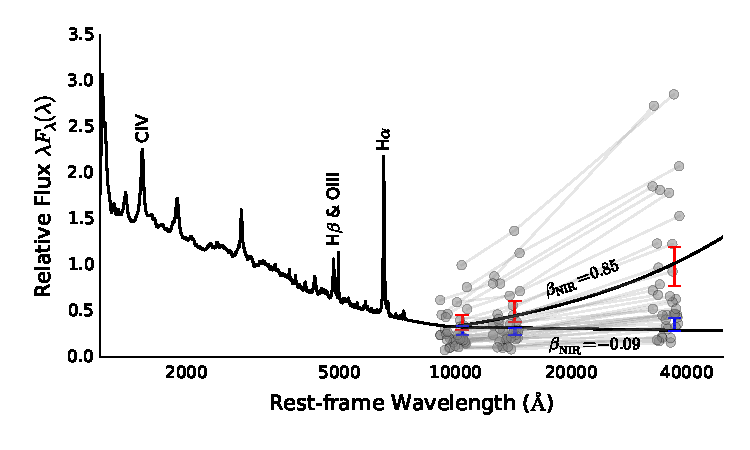
\includegraphics[width=\columnwidth]{figures/chapter06/ntt_proposal_figure2.pdf}
\caption{Representative rest-frame model spectra for the most hot-dust rich and hot-dust poor quasars in our SDSS sample, with error bars indicating the range of {\it WISE} W1, W2, and W3 magnitudes for the objects in these subsamples, transformed to the rest frame of the quasar. Grey lines show the W1, W2, and W3 fluxes for our sample of highly reddened quasars.}
  \label{fig:}
\end{figure}


Makoto Kishimoto: Slide 12 picture 

\subsection{Schemes that depend on viewing angle}

Disc emission is theoretically predicted to scale with the cosine of the disc inclination angle. 
If hot dust emission is (approximately) isotropic, the amount of hot dust emission relative to the accretion disc emission is expected to increase with increasing IA. 
However, the dust torus may block the hot dust emission at large IA \citep{roseboom13}. 
It complicates the situation and makes the dependence of $R_{NIR/UV}$ on IA uncertain. 
Runnoe et al. 2013 investiaged the inclination dependence of quasar SEDs. 
Their Figure 6 llustates that an edge on quasar spectrum tends to show a slightly enhanced NIR bump.

\citet{shen14} observed that, at fixed $R_{FeII}$, torus emission is enhanced when $FWHM_{H\beta}$ increases. 
\hbns’s width relates to the orbital velocity of gas along our line of sight. 
They conclude that \hbns's width reveals the orientation of the quasar's disc to our line of sight, with a wider line corresponding to a more edge-on disk. 
The width of other broad emission lines (e.g. \ion{Mg}{II}) should show the same dependance.   

\subsection{Dust-Free Outflow Scenario}

Correlations shown in Wang et al. and Zhang et al. could be induced by a third factor that simultaneously governs or relates to outflows and dust emission. 
Assume that hot dust emission is not directly related to outflows and is predominantly emitted by the innermost part of a hydrostatic and optically thick torus, as suggested by lots of previous studies.

1. Outflow strength is significantly dependent on the Eddington ratio, broadband SED (e.g. ionisation SED, UV continuum slope, $\beta_{UV}$) and luminosity. 
If these factors also have an impact on the hot dust emission, one might find a piece of evidence to support the dust-free outflow scenario. 
As shown in Zhang et al., Wang et al., Mor \& Trakhtenbrot, $\beta$ is almost independent of the Eddington ratio. And no correlation with luminosity. 

2. Metallicity. Quasars harboring strong outflows tend to have high gas metallicity. 
Wang et al. (2012) found that CIV blueshift increases with gas metallicity. 
Since dust forms more easily in higher metallicity gas, one may expect that metallicity is an appropriate factor which simultaneously influences outflow and hot dust emission. 
However, for a typical torus, the relative amount of dust emission is determined by the dust covering factor but not by the dust amount. 

\subsection{Dusty outflows}

BALs are on average redder than non-BAL quasars and quasars with large CIV blueshift are on average bluer than those with small blueshift. 
Since BAL and BEL outflows very likely represent the same physical component, this seeming contradiction can be reconciled by a special geometrical configuration in which dust is associated with outflows. 
In this case, dust reddening is preferably observed in the outflow direction (Wang et al.) 

Either outflows originally contain dust or dust is manufactured in outflows (Elvis et al. 2002). 

1. Dust is intrinsic to outflows. 
The idea is supported by the similar locations of BAL outflows and hot dust. 
Reverberation mapping results suggested that hot dust is located at the outer boundary of BEL regions (Suganuma et al. 2006). 
The outflow launching region is also suggested to be co-spatial with or outside of the BEL regions. 
Outflows may emerge from the outer region of the accretion disc or even the innermost region of the torus, in which the gas clouds are dusty and relatively cold. 
The dusty clouds are uplifted above the disk and are exposed to the central engine. 
The low density part is highly ionized and responsible for the blueshifted absorption and emission lines. 
Dust survives in the dense region and radiates in the NIR band. 
The dust carried by outflows is heated by the central engine to emit at the sublimation temperature, meanwhile dust absorption contributes to the outflow acceleration. 

2. Outflows interact with torus clouds. 
The process makes more dust in the clouds exposed to the central source. 
As a consequence, the IR emission increases, and the outflows become dusty. 
Since a stronger outflow can ablate dense clouds more effectively, the dependence of NIR emission on outflow strength is yielded. 
In this scenario, outflows confine the geometry and subtending angle of the dusty torus. 
One problem is that the interaction timescale is much shorter than the quasar lifetime. 
The correlation might disappear after outflows blow away all of the clouds in the outflow direction. 


Abstract paper 1: 

The \ion{C}{IV}$\lambda\lambda$1548,1550 broad emission line is visible in optical spectra to redshifts exceeding $z\sim5$. 
\ion{C}{IV} has long been known to exhibit significant displacements to the blue and these `blueshifts' almost certainly signal the presence of strong outflows.
As a consequence, single-epoch virial black hole (BH) mass estimates derived from \ion{C}{IV} velocity-widths are known to be systematically biased compared to masses from the hydrogen Balmer lines. 
Using a large sample of 230 high-luminosity ($L_{\rm Bol} = 10^{45.5}-10^{48}$ erg s$^{-1}$), redshift $1.5 < z < 4.0$ quasars with both \ion{C}{IV} and Balmer line spectra, we have quantified the bias in \ion{C}{IV} BH masses as a function of the \ion{C}{IV} blueshift. 
\ion{C}{IV} BH masses are shown to be a factor of five larger than the corresponding Balmer-line masses at \ion{C}{IV} blueshifts of 3000\kms and are over-estimated by almost an order of magnitude at the most extreme blueshifts, $\gtrsim 5000$\kms.
Using the monotonically increasing relationship between the \ion{C}{IV} blueshift and the mass ratio BH(\ion{C}{IV})/BH(\hans) we derive an empirical correction to all \ion{C}{IV} BH-masses.
The scatter between the corrected \ion{C}{IV} masses and the Balmer masses is 0.24 dex at low \ion{C}{IV} blueshifts ($\sim$0\kms) and just 0.10 dex at high blueshifts ($\sim$3000\kms), compared to 0.40 dex before the correction. 
The correction depends only on the \ion{C}{IV} line properties - i.e. full-width at half maximum and blueshift - and can therefore be applied to all quasars where \ion{C}{IV} emission line properties have been measured, enabling the derivation of un-biased virial BH mass estimates for the majority of high-luminosity, high-redshift, spectroscopically confirmed quasars in the literature. 

Abstract paper 2: 

Black-hole masses are crucial to understanding the physics of the connection between quasars and their host galaxies and measuring cosmic black hole-growth. 
At high redshift, $z \gtrsim 2.1$, black hole masses are normally derived using the velocity-width of the \ion{C}{IV}$\lambda\lambda$1548,1550 broad emission line, based on the assumption that the observed velocity-widths arise from virial-induced motions.  
In many quasars, the \ion{C}{IV}-emission line exhibits significant blue asymmetries (`blueshifts') with the line centroid displaced by up to thousands of \kms\, to the blue. 
These blueshifts almost certainly signal the presence of strong outflows, most likely originating in a disc wind.
We have obtained near-infrared spectra, including the \ha\l6565 emission line, for 19 luminous ($L_{\rm Bol} = 46.5-47.5$ erg~s$^{-1}$) Sloan Digital Sky Survey quasars, at redshifts $2 < z < 2.7$, with \ion{C}{IV} emission lines spanning the full-range of blueshifts present in the population.  
A strong correlation between \ion{C}{IV}-velocity width and blueshift is found and, at large blueshifts, $>$2000\,\kms, the velocity-widths appear to be dominated by non-virial motions. 
Black-hole masses, based on the full width at half maximum of the \ion{C}{IV}-emission line, can be overestimated by a factor of five at large blueshifts. 
A larger sample of quasar spectra with both \ion{C}{IV} and \hbns, or \hans, emission lines will allow quantitative corrections to \ion{C}{IV}-based black-hole masses as a function of blueshift to be derived. 
We find that quasars with large \ion{C}{IV} blueshifts possess high Eddington luminosity ratios and that the fraction of high-blueshift quasars in a flux-limited sample is enhanced by a factor of approximately four relative to a sample limited by black hole mass.    




On the other hand, \citet{denney13} point out that any radiatively driven wind will have a velocity comparable to the escape velocity, i.e. approximately twice the virial velocity.
Even if dominated by an outflow component, the \ion{C}{IV} line width might therefore still be expected to relate to the BH mass. 








Throughout this paper we adopt a $\Lambda$CDM cosmology with $h_0=0.71$, $\Omega_M=0.27$, and $\Omega_\Lambda=0.73$. 
Vacuum wavelengths are used for both rest-frame ultraviolet and optical features.
Unless otherwise stated, optical (i.e. SDSS) magnitudes are given in the AB system and infra-red magnitudes in the Vega system, following the conventions of the original surveys. 




\citet{denney12} presented evidence that the interpretation of the FWHM velocity of the \ion{C}{IV}-emission being due primarily to virial motions within the quasar BLR requires care.  
Specifically, both a low-velocity core component and a blue excess to the \ion{C}{IV}-emission, both of which do not reverberate, can be present and \citet{denney12} proposes that a contribution from an accretion disc wind or from a more distant narrow emission line region is important.

Changes in the \ion{C}{IV} blueshift and equivalent width are correlated with changes in the velocity widths and strengths of other optical and ultra-violet emission lines.
In the spectra of lower-redshift AGN, the FWHM of the broad \hb emission line and the relative strengths of optical \ion{Fe}{II} and \hb have been identified as the features responsible for the largest variance in the population. 
These parameters form part of `Eigenvector 1' (EV1), the first eigenvector in a principal component analysis which originated from the work of \citet{boroson92}.   
The underlying driver behind EV1 is thought to be the Eddington ratio \citep[e.g.][]{sulentic00b,shen14}. 
\citet{sulentic00} proposed a two-population model to classify AGN by their EV1 properties. 
In this scheme AGN with FWHM(\hbns) < 4000 \kms\, and FWHM(\hbns) > 4000 \kms\, are classified as population A and B objects respectively, although there is a continuous distribution of parameter values across this divide. 
\citet{sulentic07} added a measure of the \ion{C}{IV} asymmetry to EV1, and found a strong association between blue-asymmetry and their population A quasars.

\citet{denney12} found the level of contamination in single-epoch spectra from non-reverberating gas to be correlated with the shape (FWHM/$\sigma$) of the \ion{C}{IV} profile. 
\citet{runnoe13} found the scatter between the \ion{C}{IV} and \hb line widths to be correlated with the continuum-subtracted peak flux ratio of the ultraviolet emission-line blend of \ion{Si}{IV}+\ion{O}{IV} (at 1400\,\AA) to that of \ion{C}{IV}. 
Both authors used these correlations to propose empirical corrections to the \ion{C}{IV} line width which can improve the consistency between \ion{C}{IV} and \hbns-based virial BH mass estimates. 
In fact, the shape, peak flux relative to the 1400\,\AA\, blend, and blueshift of \ion{C}{IV} all correlate with one another and with other parameters in EV1.
Therefore, EV1 provides a useful context for understanding systematic trends in \ion{C}{IV} velocity widths, and hence virial BH masses. 



Much more complete coverage of the \ion{C}{IV}-emission properties within the population of luminous quasars will come from the new SDSS-IV reverberation mapping project \citep{shen15} but, for now, additional direct comparison of \ion{C}{IV}-emission and low-ionization emission-line properties in the same quasars offers a way forward.




Our aim is to directly test the reliability of \ion{C}{IV}-based BH mass estimates at high redshift for objects with a diverse range of \ion{C}{IV}-line shapes.  
In particular, we will investigate potential systematic effects on the \ion{C}{IV}-emission based BH masses for quasars with large, $\gtrsim$1200\kms, \ion{C}{IV} blueshifts, using the properties of the \ha emission line to provide BH-mass estimates for the objects unbiased by non-virial contributions to the emission-line profile.
Examining higher redshifts, our work complements other studies which attempt to improve the reliability of BH mass estimates which use the \ion{C}{IV} line \citep[e.g.][]{runnoe13,denney12}. 
However, the range of \ion{C}{IV} blueshifts in our sample is significantly more extended, which will allow us to study systematic biases in \ion{C}{IV}-based virial BH masses more directly, i.e. as a function of the \ion{C}{IV} blueshift. 
Established relations to derive BH masses from emission-line properties are employed but an advantage of our approach is that \ion{C}{IV} and \ha can be directly compared as a function of \ion{C}{IV}-emission line shape. 


While the \ion{C}{IV}-line dispersion is largely independent of the blueshift, it does not follow that dispersion-based BH-mass estimates are correct, because the underlying assumption regarding the virial-origin of the \ion{C}{IV} emission profile breaks down at large blueshifts.
Furthermore, given the difficulty in obtaining reliable dispersion measurements from survey-quality spectra with limited S/N \citep[e.g.][]{mejia-restrepo16}, virial BH-mass estimates for existing large samples of high-redshift quasars are usually based on the FWHM \citep[e.g.][]{shen11}. 
Our work therefore suggests that a viable recipe for obtaining more reliable BH mass estimates for large numbers of quasars at high redshift is to measure both the FWHM and the blueshift, which together can be used to derive a FWHM corrected for the non-virial contribution. 




Irrespective of the physical origin of the high-blueshift \ion{C}{IV}-profiles, measures of the emission-line `width' do not relate simply to virialized motions of the emitting gas under the gravitational influence of the BH. 
Excess emission-line flux in the blue wing of the \ion{C}{IV} emission increases commonly employed measures of the line-width, notably the full-width at half maximum (FWHM) and the line dispersion ($\sigma$). 
As a consequence, BH-masses derived from \ion{C}{IV} emission line velocity-widths are known to be systematically biased compared to masses from the Balmer lines \citep[e.g.][]{shen08,shen12}. 




civ fwhm trend with blueshift: This trend has previously been identified, by comparison with \ion{Mg}{II} at lower-redshifts \citep{shen08,shen11} and \hb at higher redshifts \citep{shen12}.


Significant progress in understanding the relationship between changes in \ion{C}{IV}-emission shape and quasar properties has come about through studies in which near-infrared spectra of the hydrogen Balmer lines have been obtained. 
Such studies typically involve samples of modest size and the location of the Balmer lines provides a reliable estimate of the quasar systemic redshifts; recent examples include \citet{shen12} and \citet{marziani16}. 

Throughout this paper we adopt a flat $\Lambda$CDM cosmology with $h_0=0.69$ and $\Omega_M=0.29$. 

One of the most important questions in extragalactic astronomy today is the history of supermassive black hole growth and BH/galaxy coevolution. 
Such investigations depend on acurate estimates of BH masses and accretion rates. 
This is perhaps no more obvious than in the case of the cecent claim of a 12 billion solar mass BH in the z=6.3 quasar SDSS J0100+2802 (Wu et al. 2015), which challenges our understanding of the growth of BHs. 
